\documentclass[../sparc.tex]{subfiles}
\graphicspath{{\subfix{../images/}}}
\begin{document}

%%%%%%%%%%%%%%%%%%%%%%%%%%%%%%%%%%%%%%%%%%%%%%%%%%%%%%%%%%%%%%%%%%%%%%%%%%%%%%%%
\newpage
\section{Rhythm theory}
\index{Music!Rhythm}

Our way to the music starts from the discussion of the \emph{rhythm theory}.
Most of us know that the rhythm is -- in many people it produces the reflex of
head nodding to the rhythm, or mechanical finger tapping on a tabletop to the
rhythm beats.

To understand how a rhythm is created we need to know some basic things about
the rhythm theory which will discuss below.

%%%%%%%%%%%%%%%%%%%%%%%%%%%%%%%%%%%%%%%%%%%%%%%%%%%%%%%%%%%%%%%%%%%%%%%%%%%%%%%%
\subsection{The \emph{musical bar}}
\index{Music!Rhythm!Scale}

Let's start with a musical joke: \footnote{A variation of the joke from
\url{https://www.classicfm.com/discover-music/humour/long-bar-notes-joke/}}

\begin{quotation}
C, E-flat and G walk into a bar.  The bartender says, ``Sorry, but we don’t
serve minors.''
\end{quotation}

Any musical composition is divided into time measures also known as \emph{bars}
-- usually of the same length. \footnote{Music has great variety and compositors
come up with the new tricks all the time that allow them to make the desired
impression on the listeners.  So here we are discussing the topic with some
assumptions.}

On the fig. \ref{fig:music-six-bar} we can see how could a musical composition
consisting of six bars look.

\begin{tikzpicture}
  \draw[thick, ->] (0, 0.5) -- (12, 0.5) node[anchor=north west] {t};
  \foreach \x/\n in {0/1, 2/2, 4/3, 6/4, 8/5, 10/6} {
    \draw (\x, 0) -- (\x, 1) -- (\x, 1) node[midway, above] {\n};
  };
  \label{fig:music-six-bar}
\end{tikzpicture}

The length of one bar in time is determined by the tempo of the rhythm, and we
will discuss this later.  For now, we can imagine that one one bar always takes
one abstract unit of time.  We can substitute this unit of time with any
convenient time duration -- such as one second.

Those bars are divided into smaller parts that used as cells to lay down
different sounds.  Great part of music is interweaved with mathematics, and the
first mathematical thing we face is the simple fraction.  One of the popular
ways to divide a bar is to use $\frac{4}{4}$ -- or ``four-four'' time.  In this
case a bar holds four parts, and each of which has $\frac{1}{4}$ length -- that
makes $\frac{1}{1}$ in total (or just 1.)  \footnote{There are more complicated
ways of bar division that can produce bars that are less than or more than 1 in
length.  We will talk about it later.}

If we divide a bar into four equal parts, we will get the following structure:

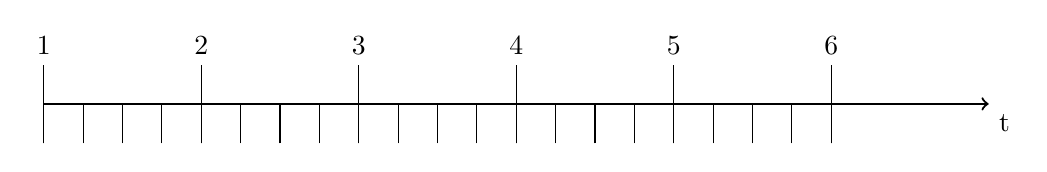
\begin{tikzpicture}
  \draw[thick, ->] (0, 0.5) -- (12, 0.5) node[anchor=north west] {t};
  \foreach \x/\n in {0/1, 2/2, 4/3, 6/4, 8/5, 10/6} {
    \draw (\x, 0) -- (\x, 1) -- (\x, 1) node[midway, above] {\n};
  };

  \foreach \x/\n in {0, 0.5, ..., 10} {
    \draw (\x, 0) -- (\x, 0.5);
  };
\end{tikzpicture}

Let's take one of the bars and investigate it closely:

\begin{tikzpicture}
  \draw[thick] (0, 0.5) -- (8, 0.5) node[anchor=north west] {t};
  \foreach \x/\n in {0/1, 8/2} {
    \draw (\x, 0) -- (\x, 1)  -- (\x, 1) node[midway, above] {\n};
  };

  \foreach \x in {0, 2, ..., 6} {
    \draw (\x, 0) -- (\x, 0.5) node[pos=0.25, right] {$ \frac{1}{4} $};
  };
\end{tikzpicture}

If we add all the parts together we will get one:

\begin{equation}
  \frac{1}{4} + \frac{1}{4} + \frac{1}{4} + \frac{1}{4} = \frac{1}{1}
\end{equation}

We can put a sound into each of the bar segments -- for now, it does not matter
if this sound is ``musical''.  Let's assume that three of the four segments will
produce a 50\gls{Hz} sound, and the last one will produce 100Hz sound:

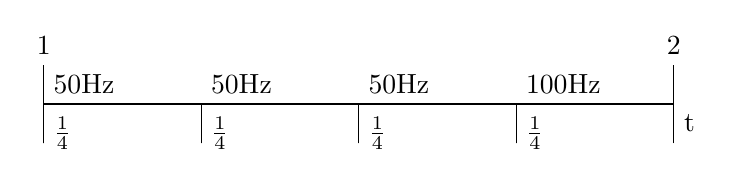
\begin{tikzpicture}
  \draw[thick] (0, 0.5) -- (8, 0.5) node[anchor=north west] {t};
  \foreach \x/\n in {0/1, 8/2} {
    \draw (\x, 0) -- (\x, 1) -- (\x, 1) node[midway, above] {\n};
  };

  \foreach \x in {0, 2, ..., 6} {
    \draw (\x, 0) -- (\x, 0.5) node[pos=0.25, right] {$ \frac{1}{4} $};
  };

  \foreach \x/\freq in {0/50, 2/50, 4/50, 6/100} {
    \draw (\x, 0) -- (\x, 0.5) node[pos=1.5, right] {\freq Hz};
  };
\end{tikzpicture}

Congratulations!  We just made a simple rhythm.  Let's program with the bar
length \texttt{T} equal to 1 second, or 1000000 microseconds.

Between the beats we should add a short delay (e.g. 100 ms) so the sounds of the
same frequency that go one after another won't be glued together.

\begin{minted}{cpp}
  // The digital port number where a speaker is connected.
  const int SPEAKER = 2;

  void setup() {
    pinMode(SPEAKER, OUTPUT);
  }

  // The procedure that generates a sound with the
  // specified parameters.
  void play_tone(int port, float f, long t) {
    const int T = 1000000 / f;
    int d = T / 2;
    int count = t / T;
    for (int i = 0; i < count; i++) {
      digitalWrite(port, HIGH);
      delayMicroseconds(d);
      digitalWrite(port, LOW);
      delayMicroseconds(d);
    }
  }

  void loop() {
    const long T = 1000000; // The length of the bar (1s)
    play_tone(SPEAKER, 50,  T / 4); // A quarter
    delay(100); // The delay between the sounds.
    play_tone(SPEAKER, 50,  T / 4); // A quarter
    delay(100);
    play_tone(SPEAKER, 50,  T / 4); // A quarter
    delay(100);
    play_tone(SPEAKER, 100, T / 4); // A quarter
    delay(100);
  }
\end{minted}

Now we can do something more complicated.

%%%%%%%%%%%%%%%%%%%%%%%%%%%%%%%%%%%%%%%%%%%%%%%%%%%%%%%%%%%%%%%%%%%%%%%%%%%%%%%%
\subsection{More complicated rhythms}

Probably some of us know this very well-known composition ``We Will Rock You''
by Queen\footnote{The official video for the composition can be found here:
\url{https://www.youtube.com/watch?v=-tJYN-eG1zk}}.

This composition has clear, easily recognizable rhythm, that in simple terms can
be described as ``two beats, one clap''.  The whole composition is built around
this rhythm -- you can perform this rhythm by making two short foot stumps on the
floor and one long clap with hands.

\begin{figure}[ht]
  \centering
  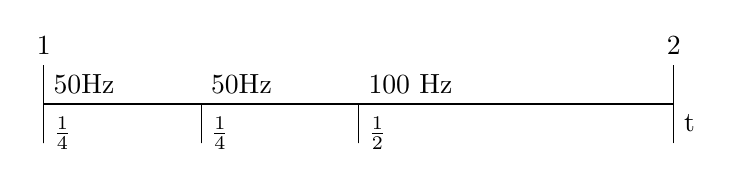
\begin{tikzpicture}
    \draw[thick] (0, 0.5) -- (8, 0.5) node[anchor=north west] {t};
    \foreach \x/\n in {0/1, 8/2} {
      \draw (\x, 0) -- (\x, 1) -- (\x, 1) node[midway, above] {\n};
    };

    \foreach \x in {0, 2} {
      \draw (\x, 0) -- (\x, 0.5) node[pos=0.25, right] {$ \frac{1}{4} $};
    };

    \draw (4, 0) -- (4, 0.5) node[pos=0.25, right] {$ \frac{1}{2} $};

    \foreach \x/\freq in {0/50, 2/50} {
      \draw (\x, 0) -- (\x, 0.5) node[pos=1.5, right] {\freq Hz};
    };
    \draw (4, 0) -- (4, 0.5) node[pos=1.5, right] {100 Hz};
  \end{tikzpicture}
  \caption{The rhythm of the melody ``We Will Rock You'' by Queen (simplified
    version.)}
  \label{fig:queen-we-will-rock-you-rhythm-1}
\end{figure}

The structure of the rhythm can be described by the sequence of simple fractions
(see fig. \ref{fig:queen-we-will-rock-you-rhythm-1}.)  The sound frequencies are
chosen by us arbitrarily.

As we can see from the fig. \ref{fig:queen-we-will-rock-you-rhythm-1}, division
of a bar don't have to be uniform -- here we have two quarters and one half.  To
add simple fractions together we have to convert them to the common denominator.
And we end up with one in the end (see the equation
\ref{equation:queen-we-will-rock-you-rhythm-1}.)

\begin{equation}
  \frac{1}{4} + \frac{1}{4} + \frac{1}{2} = \frac{1}{4} + \frac{1}{4} + \frac{2}{4} = \frac{4}{4} = \frac{1}{1} = 1
  \label{equation:queen-we-will-rock-you-rhythm-1}
\end{equation}

%%%%%%%%%%%%%%%%%%%%%%%%%%%%%%%%%%%%%%%%%%%%%%%%%%%%%%%%%%%%%%%%%%%%%%%%%%%%%%%%
\subsection{Musical rhythm notation}

From the point of the musical notation the rhythm from
fig. \ref{fig:queen-we-will-rock-you-rhythm-1} can be written down as is shown
on fig. \ref{fig:lilypond-queen-1}.

\begin{figure}[ht]
  \centering
  \begin{lilypond}
    \relative c' {
      \numericTimeSignature
      \time 4/4
      e,4 e4 e'2
    }
  \end{lilypond}
  \caption{The rhythm of the melody ``We Will Rock You'' in the musical notation
    (simplified version.)}
  \label{fig:lilypond-queen-1}
\end{figure}

We haven't discussed the musical notation yet so the figure
\ref{fig:lilypond-queen-1} can be completely obscure for us -- but don't worry,
on this stage we just have to see that there are three symbols written on the
lines.  Each symbol represents a sound of the specific length: ``\quarterNote''
($\frac{1}{4}$), ``\quarterNote'' ($\frac{1}{4}$) и ``\halfNote''
($\frac{1}{2}$).

The order of those symbols (from left to right) shows the order of playing of
those sounds, and the form of the symbol shows the length of the sound as per
the table \ref{table:music-notes-legths}.

\begin{table}[ht]
  \centering
  \def\arraystretch{2.5}%
  \begin{tabular}{|m{3cm}|m{4cm}|m{3.5cm}|}
    \hline
    \textbf{Symbol} & \textbf{Length} & \textbf{Title} \\
    \hline
    {\Large \wholeNote} & {\Large $\frac{1}{1}$} & Whole note \\[2ex]
    \hline
    {\Large \halfNote}      & {\Large $\frac{1}{2}$}  & Half-note \\[2ex]
    \hline
    {\Large \quarterNote}   & {\Large $\frac{1}{4}$}  & Quarter-note \\[2ex]
    \hline
    {\Large \eighthNote}    & {\Large $\frac{1}{8}$}  & Eighth-note \\[2ex]
    \hline
    {\Large \sixteenthNote} & {\Large $\frac{1}{16}$} & Sixteenth-note \\[2ex]
    \hline
  \end{tabular}
  \caption{Some of the possible lengths of the musical sounds (notes.)}
  \label{table:music-notes-legths}
\end{table}

There are even shorter and longer notes, but they occur less frequent than those
we listed in the table \ref{table:music-notes-legths}, so we won't discuss to
make the material more concise.

What conclusions we can make form the things we discussed above?  In the musical
notation sounds that can be ``produced'' from a musical instrument, are written
from left to right (as the regular English text.)

We can place our musical sheet on the top of a graph to make it clearer for our
understanding.  The $\mbox{X}$ axis represents the time going form left to
right:

\begin{figure}[ht]
  \centering
  \begin{lilypond}
    \relative c' {
      \numericTimeSignature
      \time 4/4
      e,4 e4 e'2
    }
  \end{lilypond}
  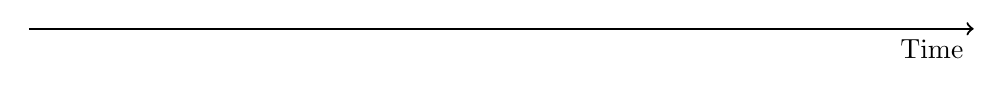
\begin{tikzpicture}
    \draw[thick, ->] (0, 0.5) -- (12, 0.5) node[anchor=north east] {Time};
  \end{tikzpicture}

  \caption{A musical ``graph''.}
  \label{fig:lilypond-queen-1}
\end{figure}

From the point of programming the source code for making such a rhythm can look
like follows:

\begin{minted}{cpp}
  // Here we skipped the previous code that does
  // the required preparations for making a sound,
  // and the implementation of "play_tone".

  void loop() {
    // The bar length in microseconds
    const long T = 1000000;

    play_tone(SPEAKER, 50, T / 4); // Quarter
    delay(100);
    play_tone(SPEAKER, 50, T / 4); // Quarter
    delay(100);
    play_tone(SPEAKER, 100, T / 2); // Half
    delay(100);
  }
\end{minted}

Now we have to figure out how to properly calculate the length of the bar to get
the lengths of its sub-divisions.

\end{document}
